%
% Verification Of Cloud Quantum Computing
%

\section{Verification of cloud quantum computing} \index{Verification}\label{sec:verification}

\subsection{Randomised benchmarking}\label{sec:rand_bench}\index{Randomised benchmarking}

\comment{Insert}

\subsection{Zero-knowledge proofs}\label{sec:ZKP}\index{Zero-knowledge proofs}

\comment{Ryan's links for NEXP ZKPs.}

\comment{General results.}

\comment{Ryan review.}

A \textit{zero-knowledge proof} (ZKP) is an interactive protocol\index{Interactive protocols} between two parties -- a \textit{prover}\index{Prover} Peggy, and a \textit{verifier}\index{Verifier} Victor -- where Peggy wishes to efficiently prove to Victor that she knows the solution to a problem, without actually revealing it. Thus, a ZKP can serve as a signature that a problem has been faithfully solved, without disclosing the solution.

ZKPs are useful in a number of cryptographic applications, most notably in authentication\index{Authentication}. In the case of classical computing, a variety of free software packages are available for compiling ZKPs for generic code. However, ZKPs become far more valuable in the case of cloud quantum computing, where there is an inherent complexity asymmetry between the client Victor (classical resources only) and the server Peggy (full quantum resources), whereby efficient ZKPs become a useful transactional tool during computational outsourcing. In a commercial context, a client can convince themselves that a server has actually performed an outsourced computation before finalising the transaction.

A conceptually simple example for illustrating the operation of a ZKP protocol is the \textit{graph isomorphism problem}\index{Graph isomorphism}. Two graphs are \textit{isomorphic}, denoted \mbox{$G_1\sim G_2$}, if there exists a permutation\index{Permutation} \mbox{$\pi\in S_n$}\footnote{In group theory\index{Group theory}, $S_n$ denotes the symmetric group\index{Symmetric group}, the set of all permutations on $n$ elements, of which there are \mbox{$|S_n|=n!$} (the order of the group).} on their vertex labels that makes them equivalent, i.e \mbox{$G_1=\pi\cdot G_2$}\footnote{Here we have employed the operator notation that \mbox{$\pi\cdot G$} means `permutation $\pi$ applied to graph $G$'. Alternately, in matrix notation, where $\pi$ is a permutation matrix and $G$ is an adjacency matrix\index{Adjacency matrix}, this operation implies the matrix conjugation\index{Conjugation} \mbox{$\pi\cdot G\cdot\pi^\top$}.}. The graph isomorphism problem is to find $\pi$ for arbitrary $G_1$ and $G_2$.

This problem is clearly contained in \textbf{NP}, since permuting vertices in graphs and directly comparing them are both computationally straightforward, making verification of the problem a polynomial-time affair. However, it is believed that explicitly determining the respective permutation is difficult in general. This is intuitively unsurprising, since for a graph with $n$ vertices, there are $n!$ possible permutations to consider (which is super-exponential), and therefore a na{\" i}ve brute-force\index{Brute-force} approach would require $O(n!)$ comparisons in the worst-case\footnote{This is the worst-case scenario. In many special cases, knowledge of underlying graph structure can simplify this enormously, yielding classically efficient runtimes.}. This problem is not believed to be contained in either \textbf{P} or \textbf{NP}-complete, and therefore presumed to be \textbf{NP}-intermediate\index{\textbf{NP}-intermediate} (Sec.~\ref{sec:introduction}).

\if 2\pubmode
\begin{figure}[!htpb]
	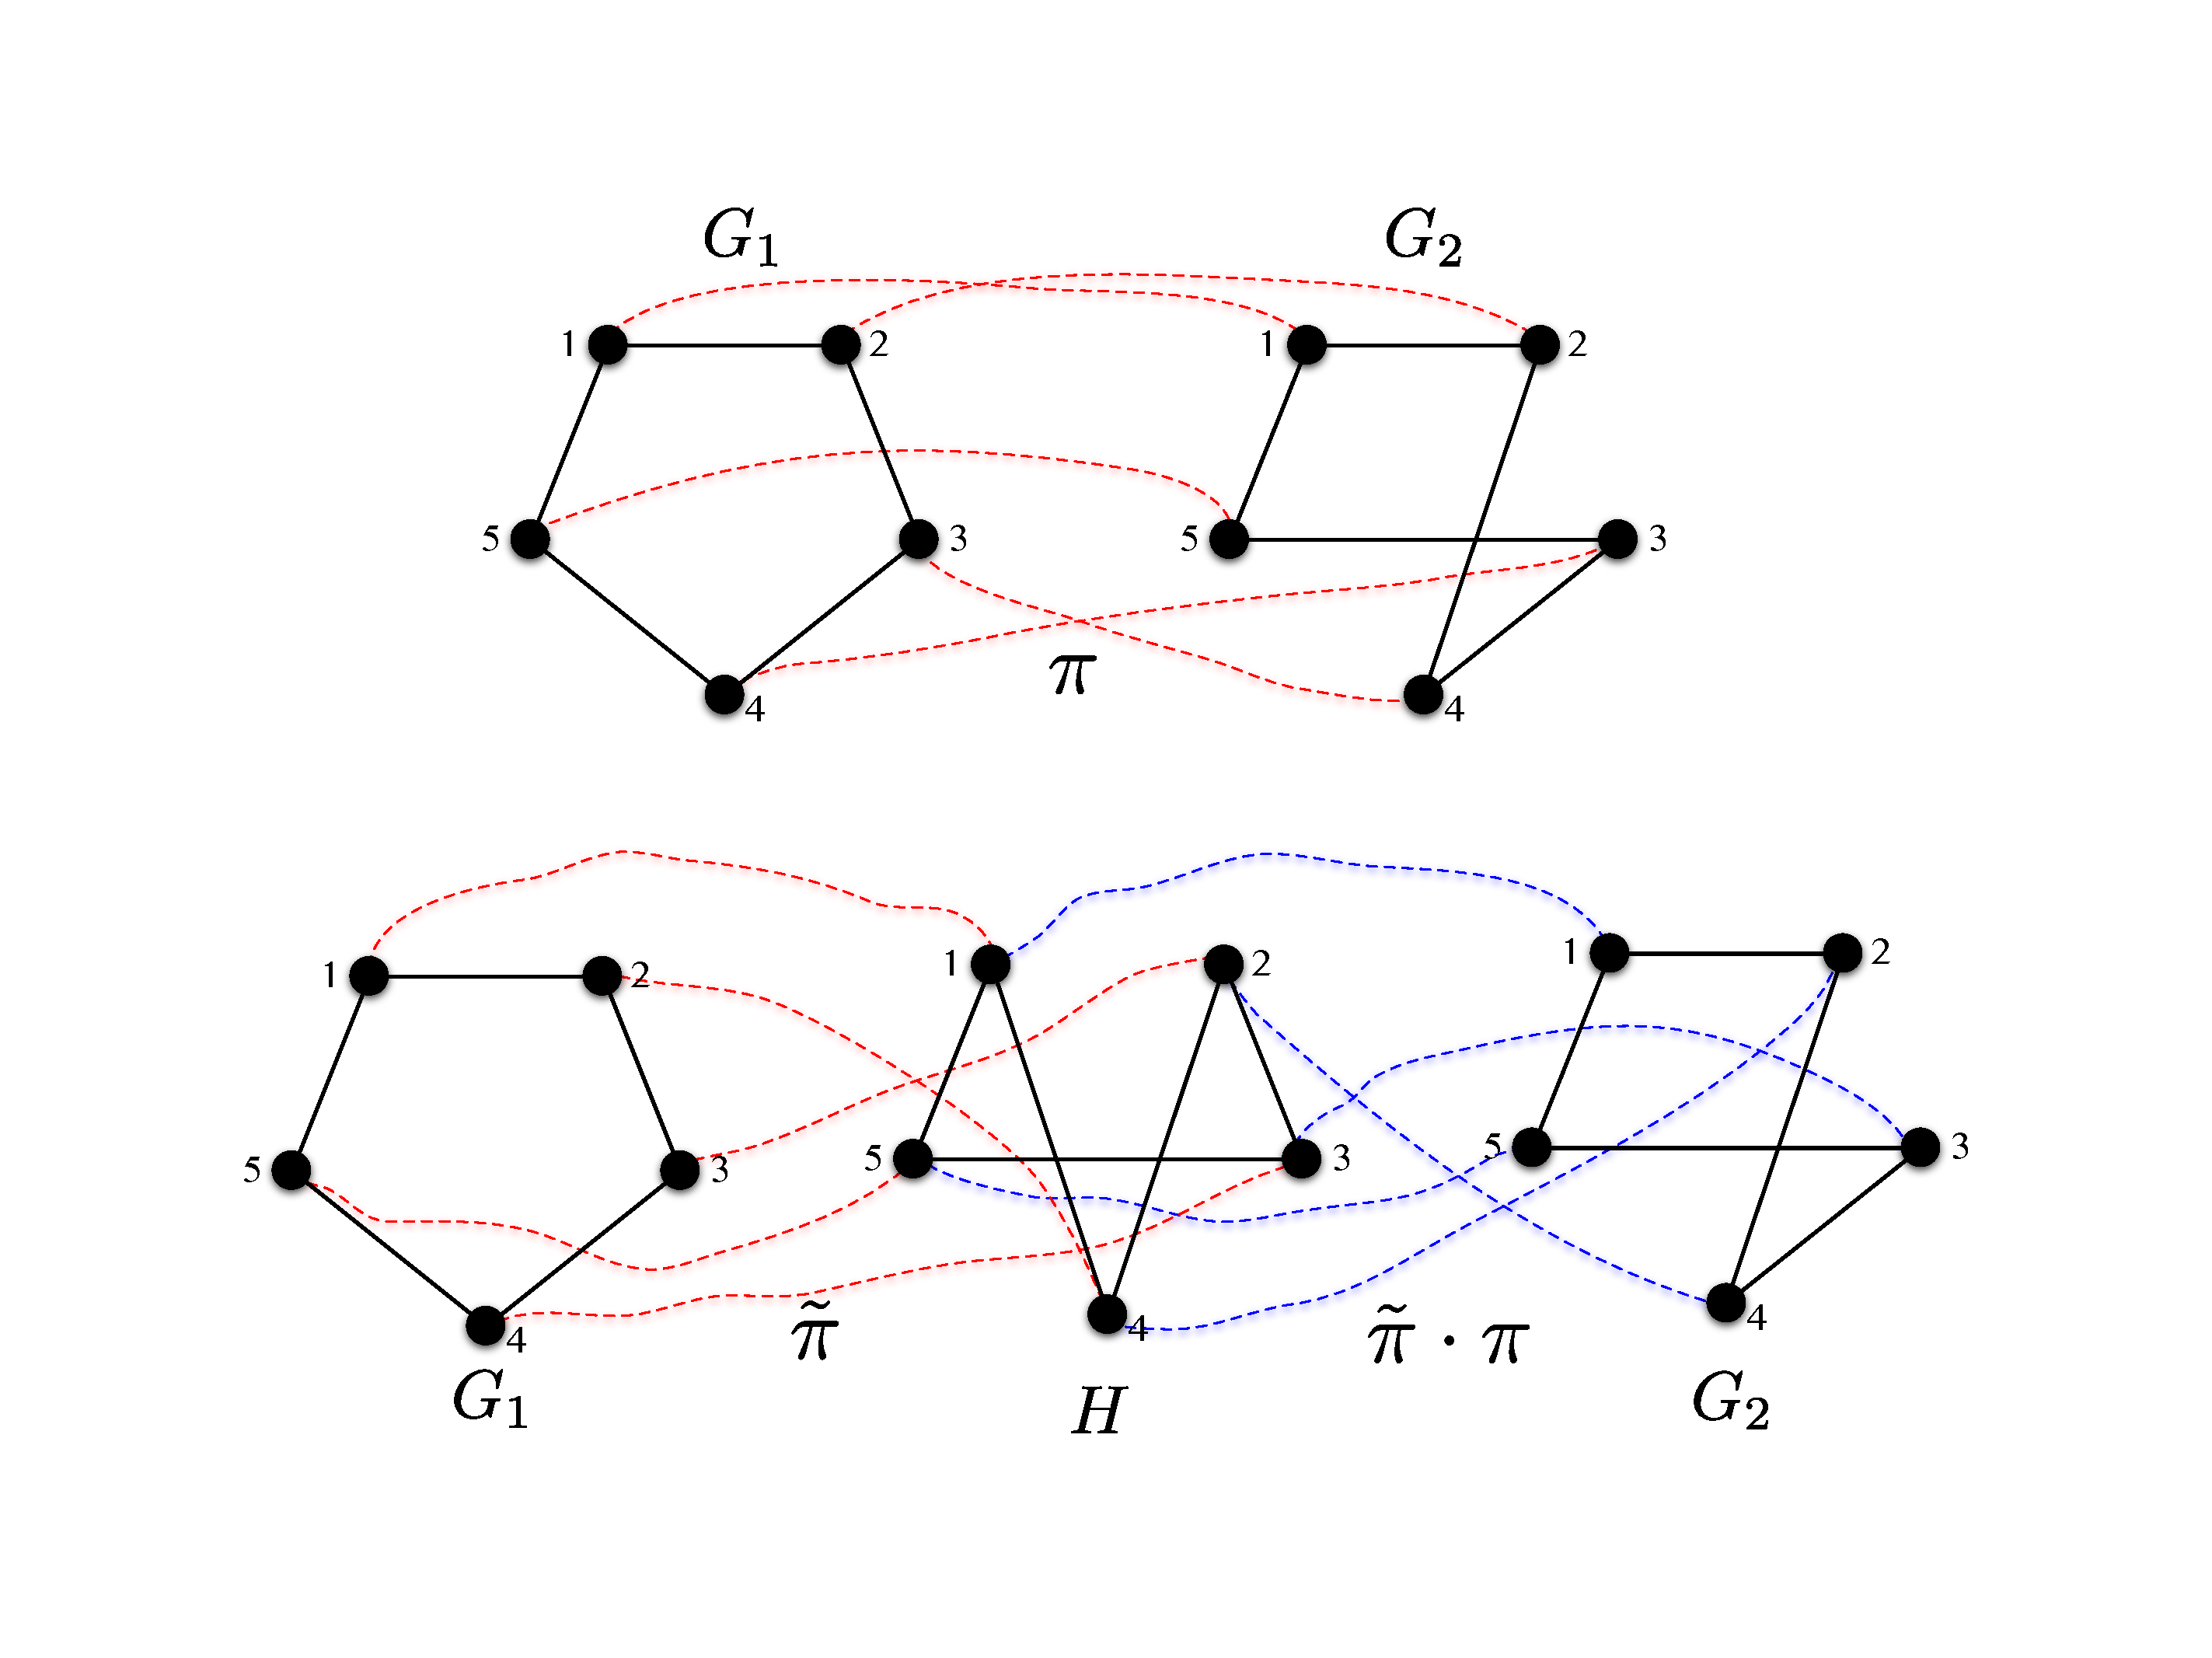
\includegraphics[clip=true, width=0.475\textwidth]{ZKP_graph_isomorphism}
\captionspacefig \caption{The isomorphisms \mbox{$G_1\sim G_2$} (top), and \mbox{$G_1\sim H\sim G_2$} (bottom). Coloured lines indicate the vertex relabelings associated with the respective isomorphisms. Knowing the latter two isomorphisms simultaneously implies knowledge of \mbox{$G_1\sim G_2$} via composition of the permutations. However, knowing only one of them does not, since $H$ is chosen randomly. By repeatedly proving knowledge of one of the isomorphisms with $H$ we achieve asymptotic certainty that the prover must have known \mbox{$G_1\sim G_2$}, without actually revealing the associated permutation.}\label{fig:ZKP_graph}
\end{figure}
\else
\begin{figure*}[!htpb]
	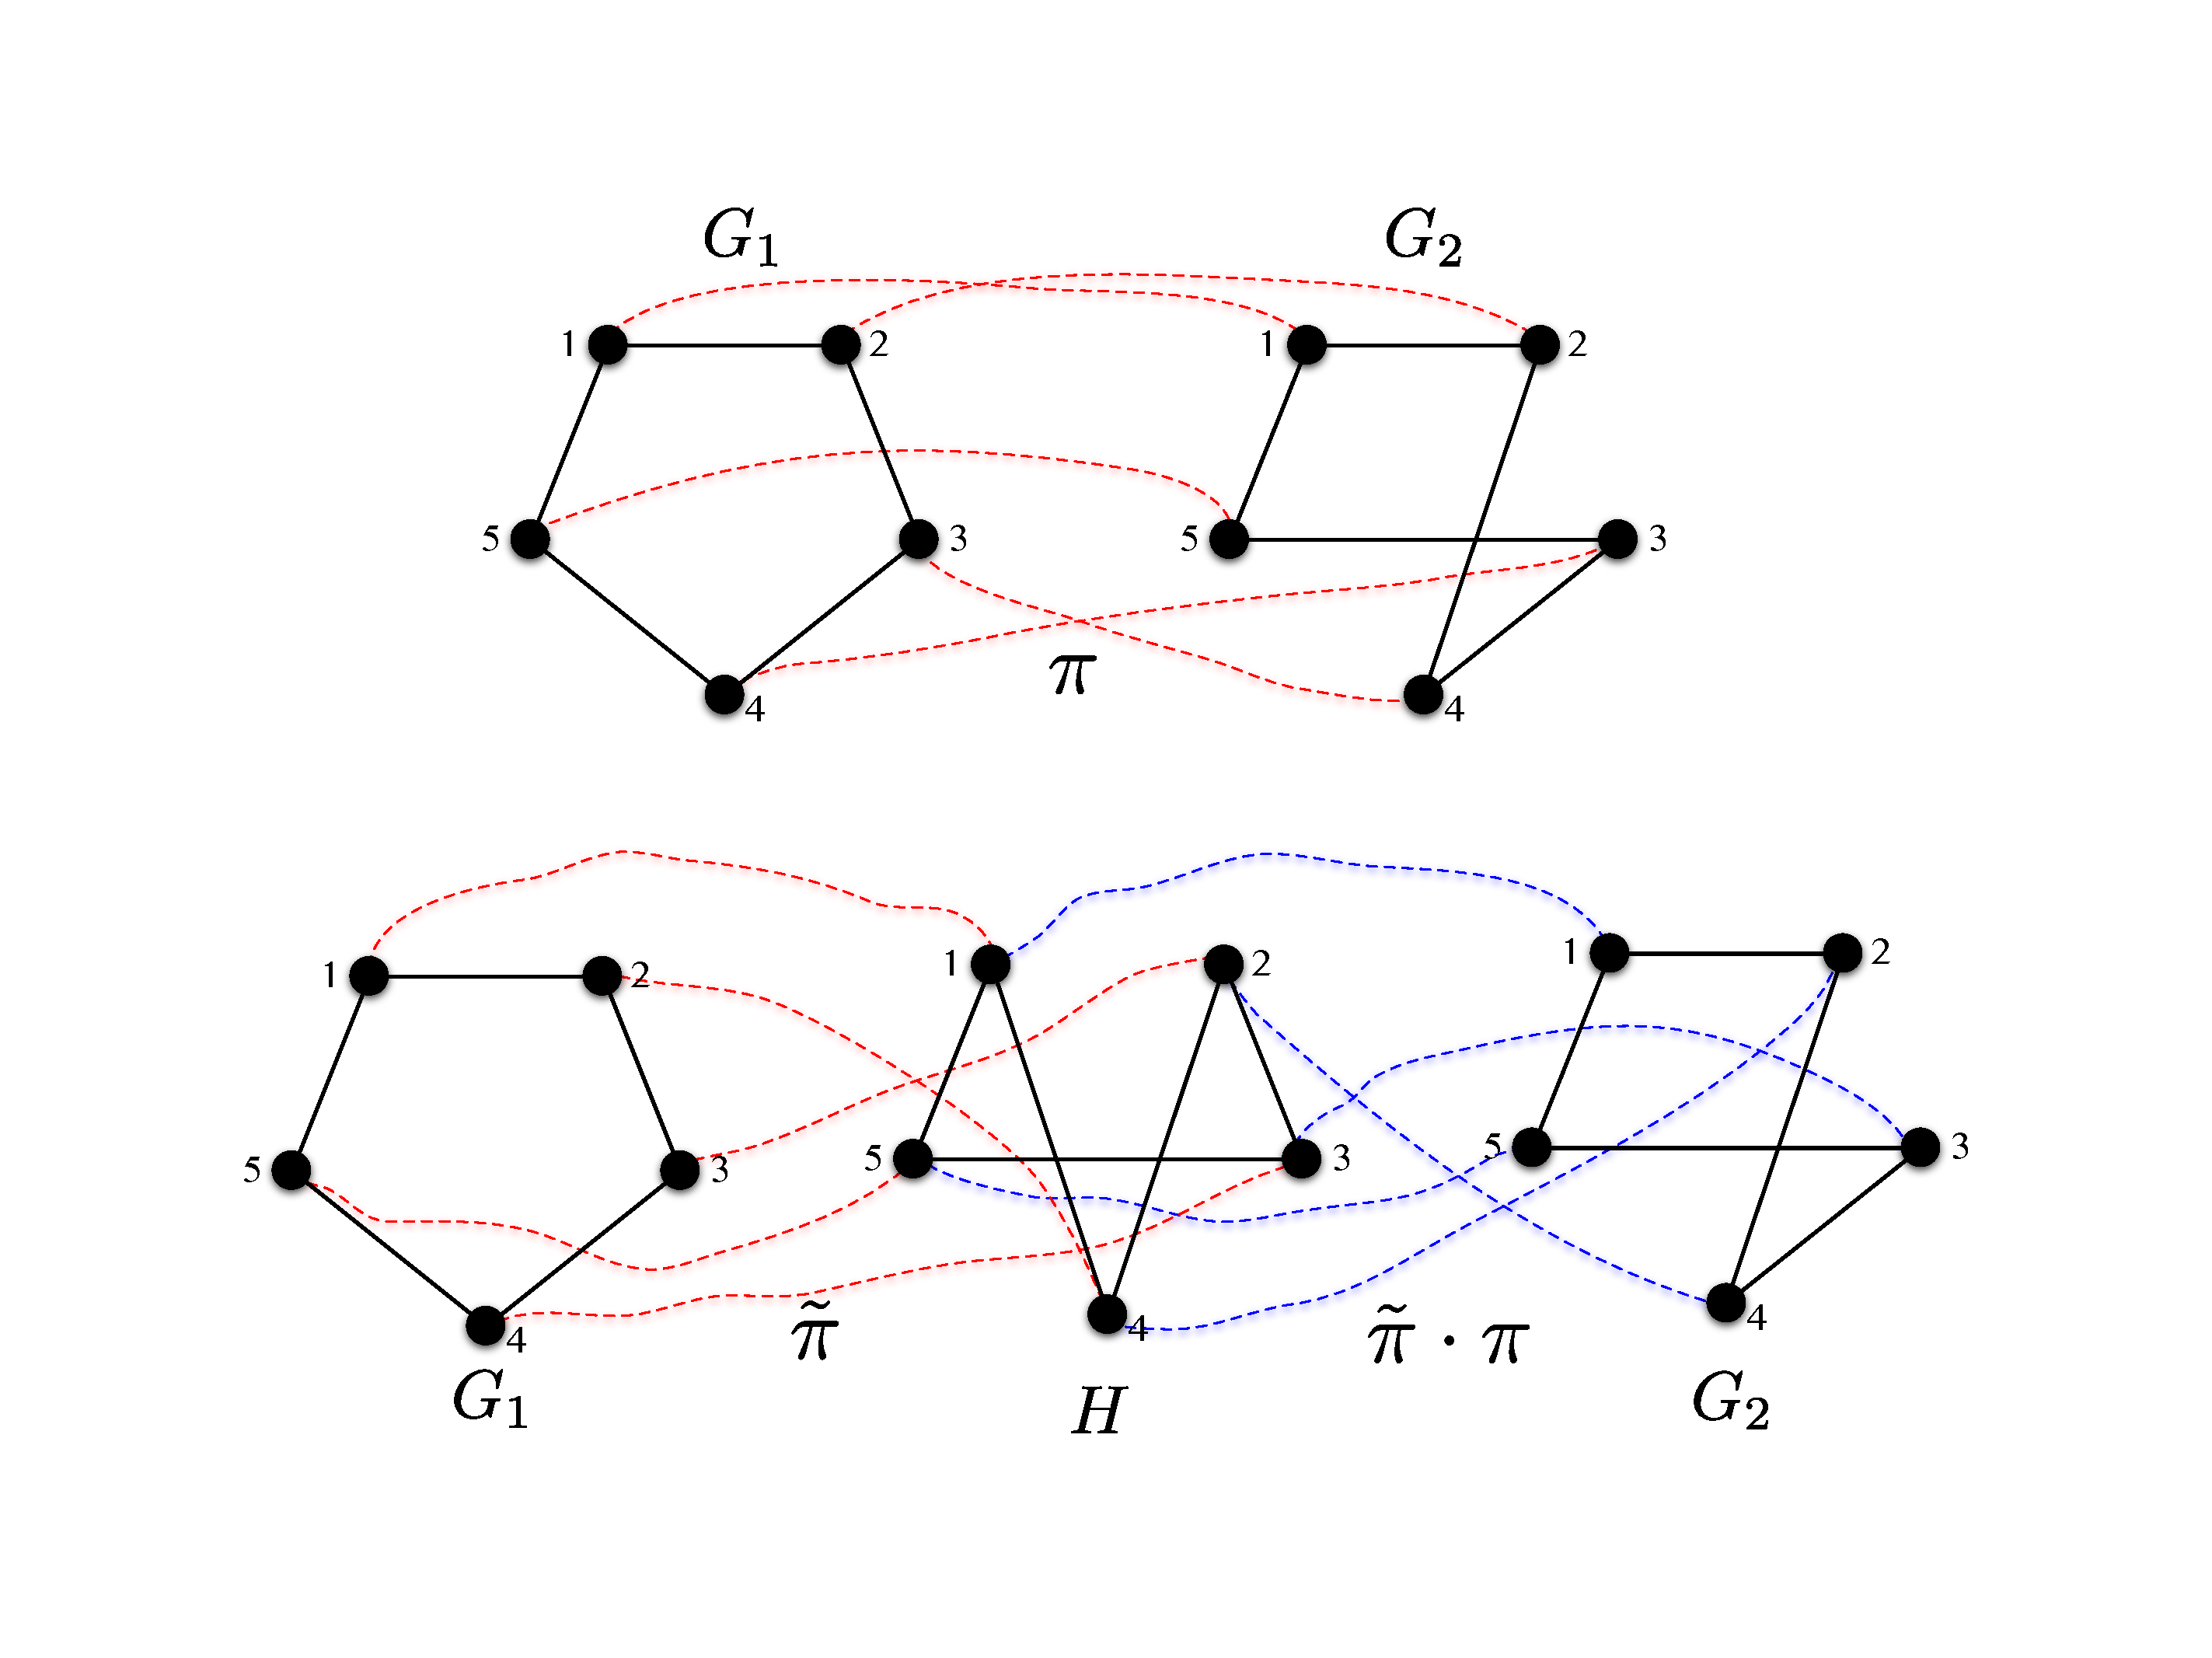
\includegraphics[clip=true, width=0.8\textwidth]{ZKP_graph_isomorphism}
\captionspacefig \caption{The isomorphisms \mbox{$G_1\sim G_2$} (top), and \mbox{$G_1\sim H\sim G_2$} (bottom). Coloured lines indicate the vertex relabelings associated with the respective isomorphisms. Knowing the latter two isomorphisms simultaneously implies knowledge of \mbox{$G_1\sim G_2$} via composition of the permutations. However, knowing only one of them does not, since $H$ is chosen randomly. By repeatedly proving knowledge of one of the isomorphisms with $H$ we achieve asymptotic certainty that the prover must have known \mbox{$G_1\sim G_2$}, without actually revealing the associated permutation.}\label{fig:ZKP_graph}
\end{figure*}
\fi

In the example isomorphism presented in Fig.~\ref{fig:ZKP_graph}(top), the vertex permutation mapping $G_1$ to $G_2$ could be expressed in vector form as,
\begin{align}
\pi = \begin{pmatrix}
	1 \\
	2 \\
	3 \\
	4 \\
	5
\end{pmatrix}_{G_1} \to \begin{pmatrix}
	1 \\
	2 \\
	4 \\
	3 \\
	5
\end{pmatrix}_{G_2},
\end{align}
where indices denote vertex labels, or equivalently via the permutation matrix,
\begin{align}
\pi = \begin{pmatrix}
	1 & 0 & 0 & 0 & 0 \\
	0 & 1 & 0 & 0 & 0 \\
	0 & 0 & 0 & 1 & 0 \\
	0 & 0 & 1 & 0 & 0 \\
	0 & 0 & 0 & 0 & 1
\end{pmatrix}.
\end{align}

\begin{table}[!htbp]
\begin{mdframed}[innertopmargin=3pt, innerbottommargin=3pt, nobreak]
\texttt{
function ZKP.GraphIsomorphism($G_1$, $G_2$):
\begin{enumerate}
	\item Graphs $G_1$ and $G_2$ are known to both verifier Victor, and prover Peggy.
	\item Peggy knows the permutation $\pi$ for the isomorphism \mbox{$G_1\sim G_2$},
	\begin{align}
		G_1 = \pi \cdot G_2.
	\end{align}
	\item Peggy wishes to prove to Victor that she knows $\pi$, without disclosing what it is.
	\item Peggy chooses another random permutation $\tilde\pi$, and constructs the new permuted graph $H$,
	\begin{align}
		H &= {\tilde\pi}\cdot G_1,\nonumber\\
		H &= {\tilde\pi}\cdot \pi \cdot G_2.
	\end{align}
	\item Peggy shares $H$ with Victor, randomly isomorphic to both $G_1$ and $G_2$.
	\item Victor randomly (\mbox{$p=1/2$}) asks Peggy to prove \textit{either} \mbox{$H\sim G_1$} or \mbox{$H\sim G_2$}.
	\item She accordingly reveals either $\tilde\pi$ or \mbox{$\tilde\pi\cdot\pi$} to Victor. He can now efficiently verify either \mbox{$H\sim G_1$} or \mbox{$H\sim G_2$} respectively, by performing the inverse permutation,
	\begin{align}
		G_1 &= {\tilde\pi}^{-1} \cdot H,\nonumber\\
		G_2 &= ({\tilde\pi}\cdot \pi)^{-1} \cdot H.
	\end{align}
	\item Victor is unable to determine $\pi$ from either scenario alone, but could were he to know \textit{both} isomorphisms simultaneously, since,
	\begin{align}
		\pi = {\tilde\pi}^{-1}\cdot (\tilde\pi\cdot\pi).
	\end{align}
	\item The above is repeated $n$ times. Each time, Peggy chooses a new random $\tilde\pi$.
	\item If Peggy does not actually know $\pi$, the probability of fraudulently passing this test $n$ times is,
	\begin{align}
		P_\text{deceive} = \frac{1}{2^n}	.
	\end{align}
	\item With confidence \mbox{$1-P_\text{deceive}$}, Victor knows that Peggy knows $\pi$, without knowing it himself.
	\item $\Box$
\end{enumerate}}
\end{mdframed}
\captionspacealg \caption{A zero-knowledge proof for the graph isomorphism problem. Victor (verifier) provides two graphs to Peggy (prover), who can demonstrate with asymptotic certainty that she knows their isomorphism, without disclosing the associated permutation relating them.} \label{alg:ZKP_graph}\index{Zero-knowledge proofs}\index{Graph isomorphism}
\end{table}

To provide a ZKP for this, Peggy's goal is to prove that she knows $\pi$, without explicitly revealing it. An efficient, randomised, classical ZKP protocol for achieving this is provided in Alg.~\ref{alg:ZKP_graph}, and a specific example illustrated in Fig.~\ref{fig:ZKP_graph}. The key underlying principle here is to obscure $\pi$ through randomisation, whereby instead of directly proving knowledge of $\pi$, it is implied via multiple proofs of isomorphisms with intermediate random graphs.